\section{Boosting To Residuals}

\begin{frame}
Let's start with our usual basic setup.\\~\\

$\{ x_i, y_i \}$ is a data set, where $i$ indexes the samples we have available for training our model.\\~\\

Each $x_i$ may be a vector, in which case I'll refer to it's components (if needed) as $x_{ij}$.\\~\\

If needed, $N$ will be the number of training samples, and $M$ the number of features.
\end{frame}
%

\begin{frame}
Our goal is to construct a function $f$ so that

$$ y_i \approx f(x_i) \ \text{for all} \ i $$

\end{frame}
%

\begin{frame}
To be more precise, let's look for an $f$ so that 

$$ \sum_i \left( y_i - f(x) \right)^2 $$

is small.
\end{frame}
%

\begin{frame}
As we saw in the introduction, we would like to build up $f$ in stages, making small adjustments as we go along.

  \begin{figure}
    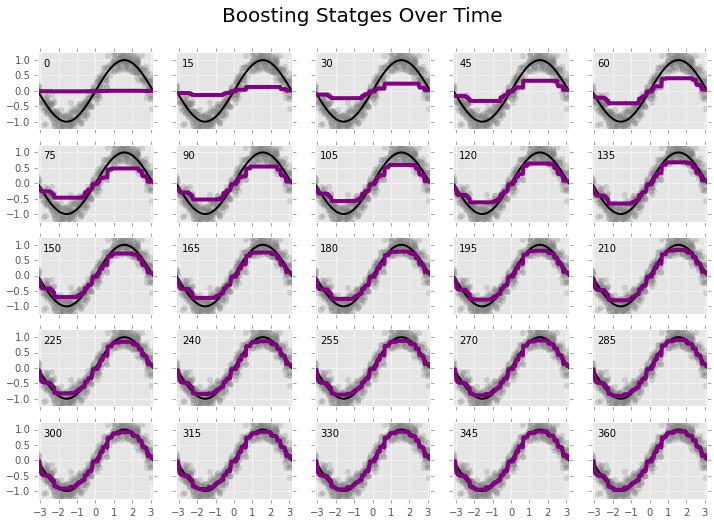
\includegraphics[scale=0.40]{boosting-over-time-multiple-plots}
  \end{figure}
  
\end{frame}
%

\begin{frame}
In the end, $f$ will be a sum of smaller (often called \textit{weak}) learners

$$ f(x) = f_0(x) + f_1(x) + f_2(x) + \cdots + f_{\text{max}}(x) $$

The process of building up the model looks like

\begin{align*}
    S_0(x) &= f_0(x) \\
    S_1(x) &= f_0(x) + f_1(x) \\
    S_2(x) &= f_0(x) + f_1(x) + f_2(x) \\
    &\vdots \\
    S_{\text{max}}(x) &= f_0(x) + f_1(x) + f_2(x) + \cdots + f_{\text{max}}(x) \\
\end{align*}
\end{frame} 
%

\begin{frame}{Where Should We Start?}
We want to make the simplest possible choice for our first stage

$$ f_0(x) = \text{constant} $$

But what constant?
\end{frame}
%

\begin{frame}
We are trying to minimize the sum of squared errors, so a good choice would be to find the constant minimizing

$$ \sum_i \left( y_i - \text{constant} \right)^2 $$

\textbf{Question}: What is the correct choice here?
\end{frame}
%

\begin{frame}
$$ f_0(x) = \frac{1}{N} \sum_i y_i $$
\end{frame}
%

\begin{frame}{How To Update}
We are now in the situation illustrated below

  \begin{figure}
    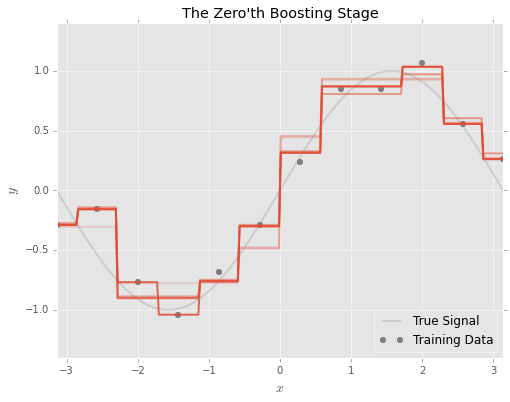
\includegraphics[scale=0.40]{zeroth-boosting-stage}
  \end{figure}

Our next task is to update our simple $f_0$ to $S_1(x) = f_0(x) + f_1(x)$.

\end{frame}
%

\begin{frame}
Intuitively, it's obvious what we should do

  \begin{figure}
    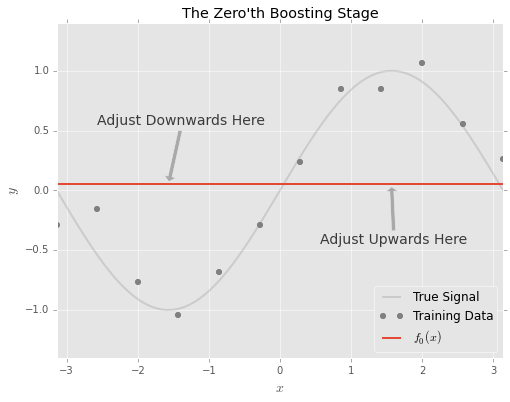
\includegraphics[scale=0.50]{zeroth-boosting-stage-what-to-do}
  \end{figure}
\end{frame}
%

\begin{frame}
But how can we use \textit{the data} to tell us this?  We won't always have the luxury of such simple pictures.

  \begin{figure}
    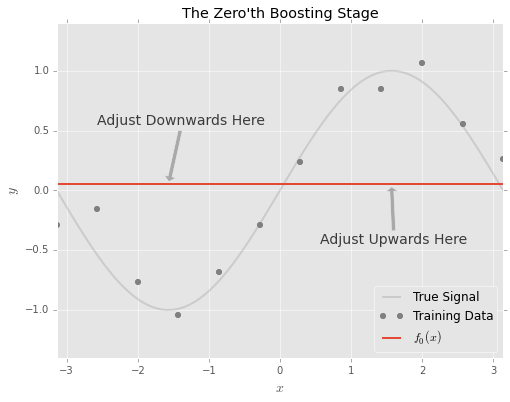
\includegraphics[scale=0.50]{zeroth-boosting-stage-what-to-do}
  \end{figure}
  
\end{frame}
%
\begin{frame}
Take a moment to think: how is the data is telling us what to do?

  \begin{figure}
    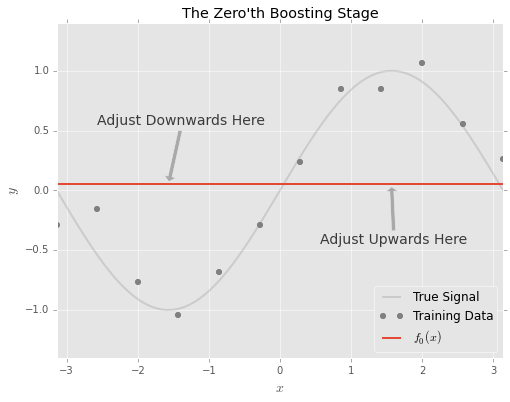
\includegraphics[scale=0.50]{zeroth-boosting-stage-what-to-do}
  \end{figure}
  
\end{frame}
%

\begin{frame}
The \textit{residuals}, $y_i - f_0(x_i)$ answer this question

  \begin{figure}
    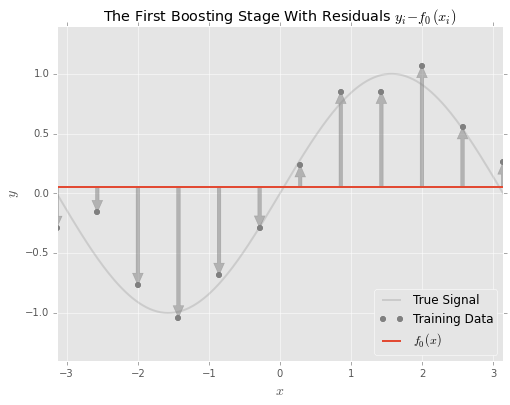
\includegraphics[scale=0.50]{first-boosting-stage-with-residuals}
  \end{figure}
\end{frame}
%

\begin{frame}
  \begin{center}
    \textbf{We should adjust $f_0(x)$ in the direction of the residuals!}\\~\\
  \end{center}

\only<2>{
  \begin{center}
    But...  there is a huge issue with this...
  \end{center}
}

  \begin{figure}
    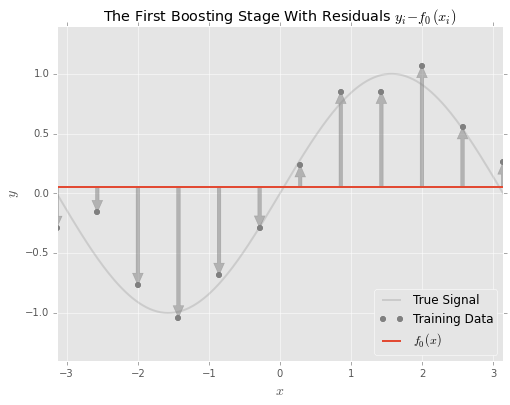
\includegraphics[scale=0.50]{first-boosting-stage-with-residuals}
  \end{figure}
  
\end{frame}
%

\begin{frame}

  \begin{figure}
    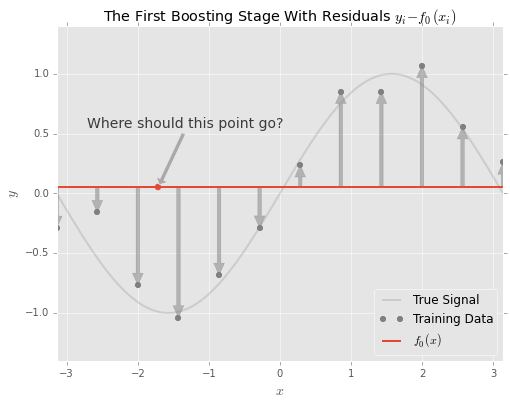
\includegraphics[scale=0.60]{first-boosting-stage-with-residuals-dillema}
  \end{figure}
  
\end{frame}
%

\begin{frame}
We can only calculate residuals \textit{at the training data points}!

  \begin{figure}
    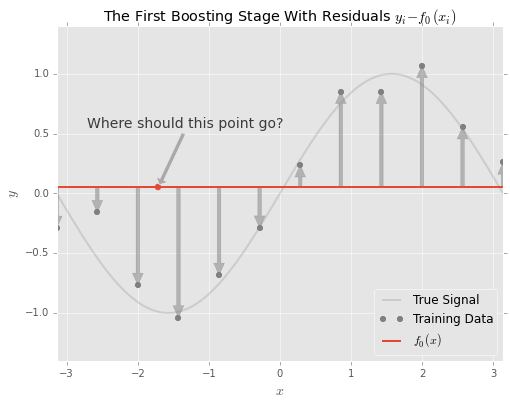
\includegraphics[scale=0.40]{first-boosting-stage-with-residuals-dillema}
  \end{figure}

We need some way of \textbf{extending} the values of the residuals to places we \textit{do not have data}.
\end{frame}
%

\begin{frame}
\textbf{Solution:}\\~\\

\only<2->{Fit a model to the residuals!\\~\\}

\only<3->{
  The \textbf{predictions from this model} both:
  \begin{itemize}
    \item Approximate the residuals at the places we \textit{have} data.
    \item Are defined everywhere.
  \end{itemize}
}
\end{frame}
%

\begin{frame}
Here is a \textit{new} dataset.

\begin{itemize}
  \item The values of $x$ are the same as before, taken directly from the training data.
  \item The response values are the \textit{residuals}: $y_{\text{new}} = y_i - f_0(x_i)$.
\end{itemize}

  \begin{figure}
    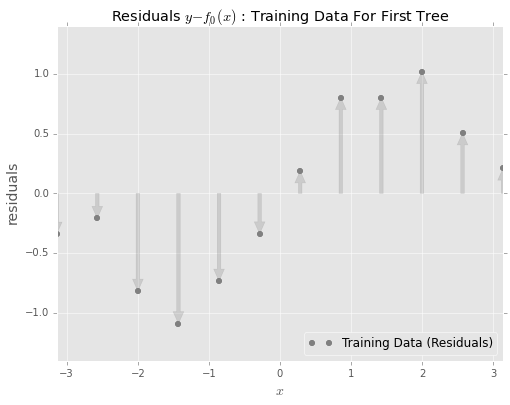
\includegraphics[scale=0.40]{first-boosting-stage-residual-training-set}
  \end{figure}
  
\end{frame}
%

\begin{frame}
Here is a very simple model fit to this \textit{working data set}

  \begin{figure}
    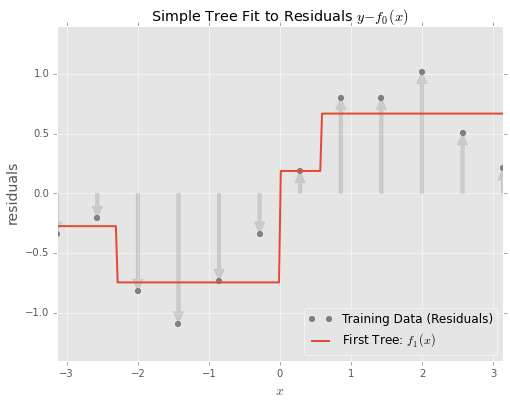
\includegraphics[scale=0.50]{first-boosting-stage-residuals-with-tree}
  \end{figure}

\end{frame}
%

\begin{frame}
Now we can update the model.

$$S_1(x) = f_0(x) + f_1(x) \leftarrow \text{Model fit to residuals!}$$

  \begin{figure}
    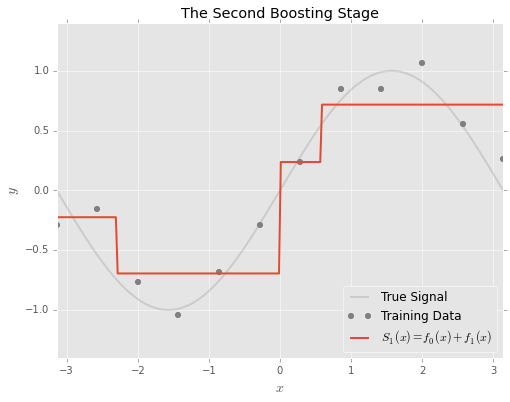
\includegraphics[scale=0.40]{second-boosting-stage}
  \end{figure}
  
\end{frame}
%

\begin{frame}
  \begin{center}
    Let's go one more step, so that the idea is clear.
  \end{center}
\end{frame}
%

\begin{frame}
Calculate the residuals of the current model...

  \begin{figure}
    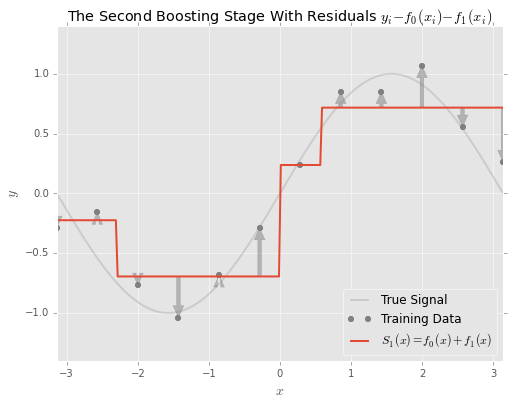
\includegraphics[scale=0.50]{second-boosting-stage-with-residuals}
  \end{figure}
  
\end{frame}
%

\begin{frame}
Create a training data set with the residuals as the response...

  \begin{figure}
    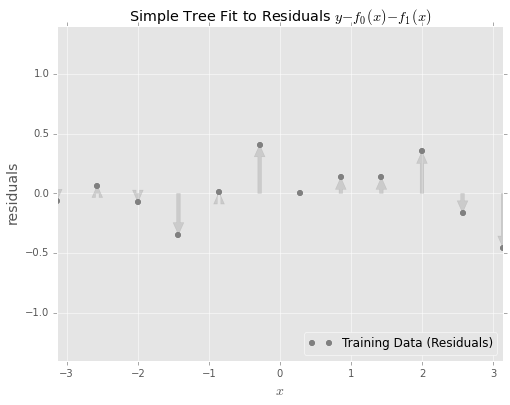
\includegraphics[scale=0.50]{second-boosting-stage-residual-training-set}
  \end{figure}
  
\end{frame}
%

\begin{frame}
Create a training data set with the residuals as the response...

  \begin{figure}
    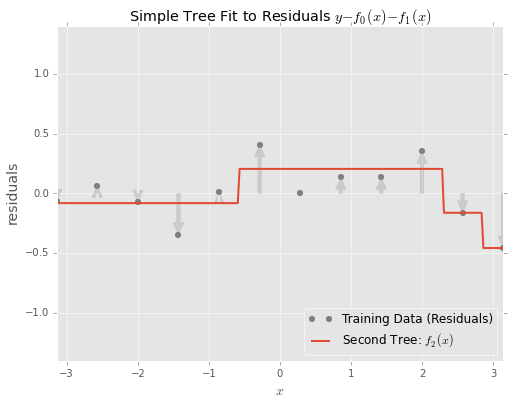
\includegraphics[scale=0.50]{second-boosting-stage-residuals-with-tree}
  \end{figure}
  
\end{frame}
%

\begin{frame}
Update the model!

  \begin{figure}
    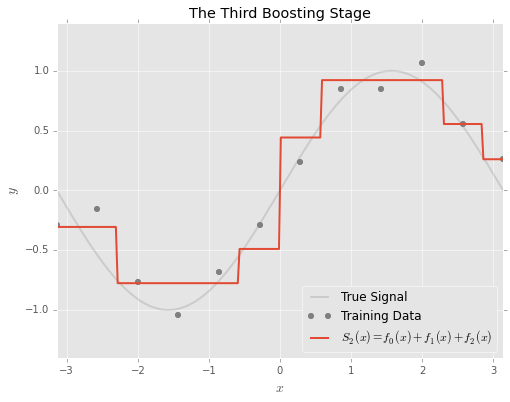
\includegraphics[scale=0.50]{third-boosting-stage}
  \end{figure}
  
\end{frame}
%

\begin{frame}

  \begin{figure}
    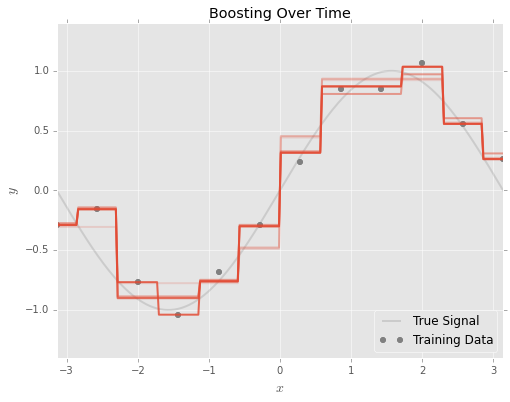
\includegraphics[scale=0.60]{simple-boosting-over-time}
  \end{figure}
  
\end{frame}
%

\begin{frame}{But, What Happened to Growing Slowly Over Time?}
Instead of adding in the entirety of the residual fitted tree during an update

$$ S_{k+1}(x) = S_{k}(x) + f_{k+1}(x) $$

Instead we added some \textit{small fraction} of $f_{k+1}$

$$ S_{k+1}(x) = S_{k}(x) + \lambda f_{k+1}(x) $$
\end{frame}
%

%

\begin{frame}
$$ \lambda = 0.01 $$

  \begin{figure}
    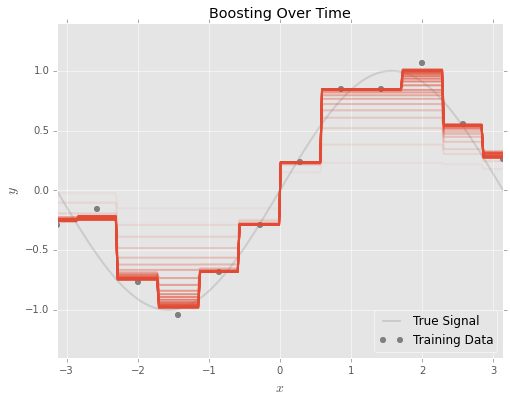
\includegraphics[scale=0.50]{simple-boosting-over-time-learning-rate}
  \end{figure}

\end{frame}
%

\begin{frame}{Gradient Boosting to Minimize Sum of Squared Errors}

\textbf{Inputs:} A data set $\{ x_i, y_i \}$, and a learning rate $\lambda$.

\textbf{Returns:} A function $f$ such that $f(x_i) \approx y_i$.

\begin{itemize}
  \item Initialize $S_0(x) = f_0(x) = \frac{1}{N} \sum_i y_i$.
  \item Iterate (parameter $k$) until satisfied: \begin{itemize}
    \item Create the working data set $W_k = \{ x_i, y_i - S_{k-1}(x_i) \}$.
    \item Fit a decision tree to $W_k$, minimizing least squares.  Call this tree $f_k$.
    \item Set $S_{k+1}(x) = S_{k}(x) + \lambda f_{k}(x)$. 
  \end{itemize}
  \item Return $f_{\text{max}}(x) = f_0(x) + f_1(x) + f_2(X) + \cdots + f_{\text{max}}(x)$.
\end{itemize}

\end{frame}
%

\begin{frame}{Why is it Called Gradient Boosting?}
Remember when we were in this situation:

  \begin{figure}
    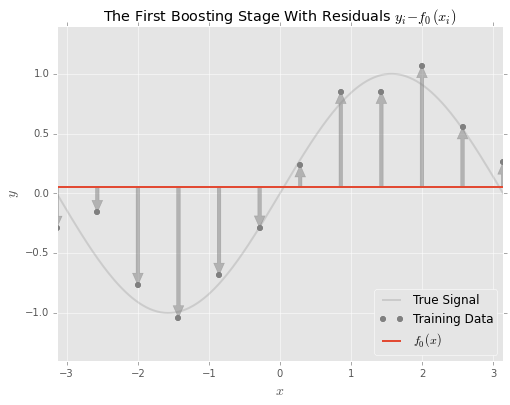
\includegraphics[scale=0.35]{first-boosting-stage-with-residuals}
  \end{figure}
  
We want to use the residuals to update the model

$$ S_{k+1}(x_i) = S_{k}(x_i) + \lambda (y_i - S_{k}(x_i)) $$

\end{frame}
%

\begin{frame}
Removing the details of the specific situation, this looks like

$$ S_{k+1}(x_i) = S_{k}(x_i) + \lambda (y_i - S_{k}(x_i)) $$
$$ \Downarrow $$
$$ \xi_{k+1} = \xi_k + \lambda (y - \xi_k) $$

\textbf{Question:} Does this look... familiar?
\end{frame}
%

\begin{frame}

\only<1>{
\textbf{Recall}: Gradient descent is a general purpose algorithm for optimizing any objective function $L(x)$.\\~\\

  \begin{center}
    \textit{How does this go?}
  \end{center}
}

\only<2>{
\textbf{Algorithm:} Gradient Descent to Minimize a function $L$.\\~\\

\textbf{Inputs:} A function $L$.

\textbf{Outputs:} A point $x_{\text{optim}}$ that minimizes $L$. \\~\\

\begin{itemize}
  \item Compute $\nabla L(x)$ somehow, on paper is good.
  \item Initialize $x_0 = 0$ (arbitrary, there may be more principled choices).
  \item Iterate until convergence: \begin{itemize}
    \item Set $x_{i+1} = x_i - \lambda \nabla L(x_i)$.
  \end{itemize}
\end{itemize}
}

\end{frame}
%

\begin{frame}
What happens when we apply gradient descent to minimize the squared error loss?

$$ L(\xi, y) = \frac{1}{2} \left( y - \xi \right)^2 $$
\end{frame}
%

\begin{frame}
$$ - \nabla_{\xi} L (\xi, y) = - \frac{1}{2} \frac{\partial}{\partial \xi} \left( y - \xi \right)^2 = y - \xi $$
\end{frame}
%

\begin{frame}
So gradient descent for least squares looks like...

$$\xi_{k+1} = \xi_{k} - \lambda \nabla_{\xi} L (\xi_k, y) = \xi_{k} + \lambda (y - \xi_{k})$$

That is, \textbf{least squares gradient descent iteratively moves in the direction of the residual}.
\end{frame}
%

\begin{frame}
This is why the algorithm is called \textbf{Gradient Boosted Regression}.\\~\\

We "boost" the current estimate by adding an \textit{approximation to the gradient of the squared error loss function}.
\end{frame}

